\section{Аналитический раздел}

\subsection{Понятие самоубийства и суицидального поведения}
Самоубийство -- это умышленное лишения себя жизни. \cite{fuckingSuicideDefinition}

На каждое самоубийство приходится гораздо больше несостоявшихся суицидентов, каждый несостоявшийся факт самоубийства является важным фактором риска самоубийства среди населения в целом. \cite{suicideVOZDouble}

Суицидной считается любая внутренняя либо внешняя активность, движимая стремлением человека лишить себя жизни. Внутренняя форма проявления суицидального поведения включает в себя пассивные суицидальные мысли, замыслы и намерения, а также соответствующий эмоциональный фон -- суицидальные переживания. Внешнее суицидальное поведение проявляется в виде суицидальных практических суицидальных действий или высказываний, включая использование средств и способов, которые  итоге могут привести к самоустранению или провоцировать его попытку. \cite{suicidalContent}

Существует три типа суицидального поведения \cite{Kasyanov}:
\begin{itemize}
\item самоубийство как решение проблемы (например, "если я умру, то больше не будет никаких проблем");
\item самоубийство как цель, желание (например, "я хочу умереть");
\item саморазрушительное поведение (например, нанесение себе увечий).
\end{itemize}

Одной из самых уязвимых в плане суицидальной активности категорий являются подростки и молодежь. Более половины попыток суицида подростков являются демонстративными, но различить истинные и демонстративные суицидные попытки -- одна из сложнейших задач. По клиническим данным, примерно каждый третий случай завершенного суицида сопровождается не до конца известной мотивацией. \cite{suicidalContent}

Суицидальное поведение может интерпретироваться как просьба о помощи в 90\% случаев, и лишь в 10\% случаев -- как истинное желание покончить с собой. \cite{Kasyanov}

\subsection{Предотвращение самоубийств}

Существует связь между совершением или планированием самоубийства и психическими расстройствами, такими как депрессия или алкоголизм. Кроме того, к группе риска относятся люди, уже совершавшие попытки суицида. Однако многие самоубийства совершаются импульсивно в кризисные моменты, сопровождающиеся неспособностью справляться с жизнью, стрессом, финансовыми проблемами, хроническими болезнями или разрывом отношений. С суицидальным поведением тесно связаны и переживания конфликтов, катастроф, насилия, жестокого обращения или утраты или чувство изоляции, возникающее у групп, подвергающихся дискриминации. \cite{suicideVOZDouble}

Самоубийства предотвратимы, для этого существует ряд мер, которые предполагают вмешательства, основанные на фактических данных \cite{suicideVOZDouble}:

\begin{itemize}
	\item ограничение доступа к средствам самоубийства (пестицидам, огнестрельному оружию, лекарствам);
	\item взаимодействие со средствами массовой информации для ответственного освещения случаев самоубийств;
	\item развитие социально-эмоциональных жизненных навыков у подростков и уязвимых групп;
	\item раннее выявление, оценка и наблюдение за уязвимыми группами.
\end{itemize}

Ключевой проблемой борьбы с ростом числа самоубийств является ``стигма'', которая определяется как отсутствие обращений за помощью людей, думающих о суициде, или совершавшие попытку покончить жизнь самоубийством. Такие люди не получают должной помощи. Кроме того, во многих сообществах существует запрет на открытое обсуждение данных вопросов. \cite{suicideVOZDouble}

\subsection{Статистика самоубийств}
Каждый год в мире совершается 703 000 самоубийств и еще больше попыток самоубийств. Данные акты происходят не только в странах с высоким уровнем дохода, но и являются глобальным явлением во всех регионах мира. \cite{suicideVOZDouble}

В период с 2010 по 2021 год уровень самоубийств увеличился примерно на $36\%$. В 2021 году самоубийства стали причиной 48 183 смертей, также $12.3$ миллиона взрослых американцев серьезно думали о самоубийстве, $3.5$ миллиона планировали попытку самоубийства, а $1.7$ миллионов человек пытались покончить жизнь самоубийством. \cite{suicideStats}

На каждую смерть от самоубийства в 2021 году приходилось около \cite{suicideStats}:
\begin{itemize}
	\item 3 госпитализации по причине членовредительства;
	\item 8 обращений в отделение неотложной помощи в связи с самоубийством;
	\item 38 попыток самоубийства, о которых сообщили сами люди за последний год;
	\item 265 человек, которые всерьез задумывались о самоубийстве за последний год. 
\end{itemize}

Также стоит отметить, что уровень самоубийств среди мужчин в 2021 году был примерно в 4 раза выше, чем среди женщин. Таким образом $50\%$ населения является $80\%$ самоубийц. Самый высокий же уровень самоубийств по возрасту наблюдается у людей старше 85 лет, а наиболее распространенным методом сведения счетов с жизнью -- огнестрельное оружие.

Статистика количества суицидов в определенные месяцы года представлена на рисунке \ref{img:cdcsuicides} \cite{suicideStats}.

\begin{figure}[H]
	\centering
	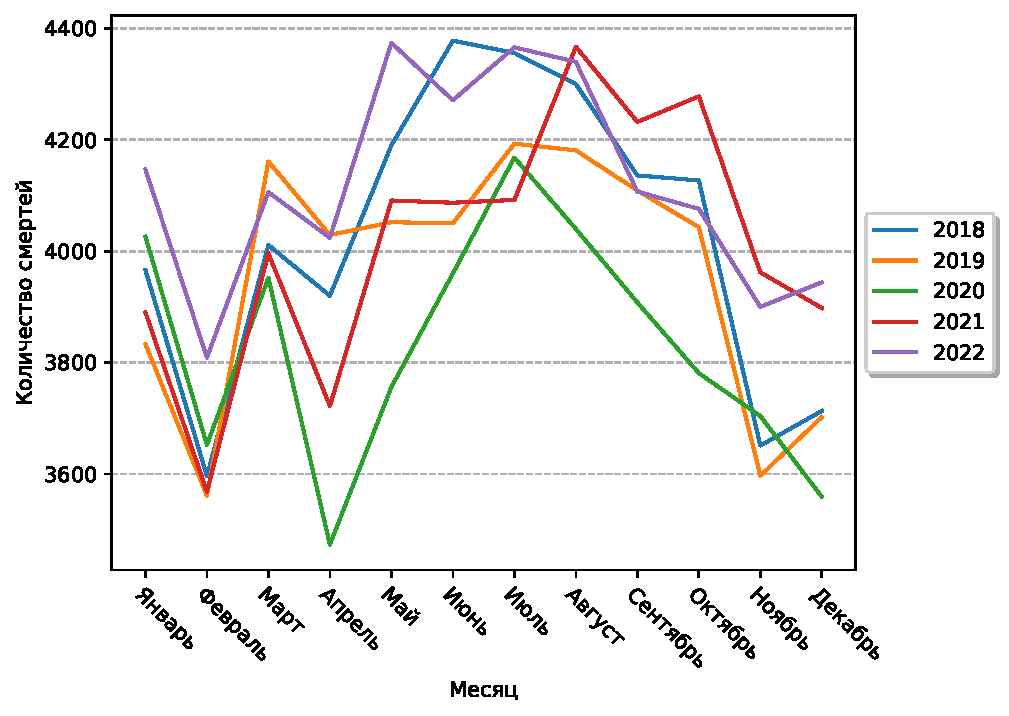
\includegraphics[width=\textwidth]{inc/deathToMonth.pdf}
	\caption{ График количества смертей от суицида в определенные месяцы за 2018--2022 год. }
	\label{img:cdcsuicides}
\end{figure}


\subsection{Классификация признаков паттернов суицидального поведения человека}

Признаки паттернов суицидального поведения человека по своей форме проявления могут быть явными и неявными. К явным признакам суицидального поведения относятся просьбы о помощи, в то время как к неявным -- намеки на собственное состояние, депрессивные высказывания, изоляция от общества.

Кроме того, каждая форма проявления, как просьба о помощи, может выражаться:

\begin{itemize}
	\item аудиально -- с использованием речевого аппарата, интонаций, музыкальных композиций;
	\item в текстовом виде -- записка или сообщение;
	\item визуально -- с использованием собственного имиджа, жестов, паттернов движений;
	\item социально -- через изоляцию или конфликты с обществом;
	\item физиологически -- затяжная депрессия, приводящая к суицидальным наклонностям, сказывается на организме человека.
\end{itemize}

В сети интернет наиболее доступными являются явные и неявные признаки, выражающиеся в текстовом виде, причем в качестве анализируемого материала могут использоваться как личные сообщения, так и предоставляемые широкому кругу лиц тексты с описанием жизненных ситуаций, собственного состояния или личных переживаний.

\subsection{Форматы хранения проявление поведения человека}

Для автоматизации анализа выражений форм проявления суицидального поведения человека и выявления патологий требуется определить формат хранения данных.

Результатом анализа \textit{аудиальных признаков} может быть наличие в словах человека депрессивных высказываний или интонаций пользователя в разговоре, умеющем суицидальный подтекст. Анализ аудио-сообщений подразумевает их расшифровку и сопоставление определенных высказываний с проявляемыми эмоциями. Далее под ``эмоциональной картой аудио-дорожки'' имеется в виду структура, в которой для определенных аудио-фрагментов сопоставлена одна из рассматриваемых эмоций пользователя. Данная структура может быть представлена как временные промежутки аудио-сообщения или как указатель на части расшифровки. 

Результатом анализа  \textit{текстовых сообщений} может быть наличие в сообщении каких-либо суицидальных признаков: употребление выражений, подразумевающих суицидальную тематику, слова с суицидальным подтекстом, прямые высказывания о желании совершить суицид.

Результатом анализа \textit{пространственно-временных признаков} может быть как выявление подверженности жителей определенных регионов депрессии в связи с происходящими в них событиями, или же соотнесение временных промежутков цикличным сезонам депрессии.

Результатом анализа \textit{визуальных признаков} может быть определение проявления суицидального поведение, попытки суицида, либо его совершение, а также определение депрессии по мимике во время высказываний. Анализ визуальных признаков подразумевает обработку видеозаписей с действиями человека.

\textit{Социальные признаки} могут выражаться как действия самого человека в социальной сфере или же информация, поступающая из социальной среды исследуемого индивидуума. Результатом анализа данных признаков может быть установление факта социальной изоляции исследуемого человека, либо встревоженность окружения: родственников, друзей или знакомых. Анализ подразумевает мониторинг социальных связей человека или сбор данных о наблюдениях окружающих индивидуума людей.

Анализ \textit{физиологических признаков} может включать в себя либо диагностику депрессивного состояния, либо частотность присутствия индивидуума в стрессовых ситуаций, которые сопровождаются стадией истощения организма. \textit{Общий адаптационный синдром} --- это сочетание стереотипных реакций, возникающих в организме в ответ на действие стрессоров и обеспечивающих ему устойчивость не только к стрессорному агенту, но и по отношению к другим болезнетворным факторам \cite{stressAndPatology}. Определены три стадии общего адаптационного синдрома: тревоги, ус\- тойчивости и истощения. При длительном воздействии стрессора адаптивные механизмы, участвующие в поддержании резистентности, исчерпывают себя, и наступает стадия истощения организма. Данная стадия не является обязательной и стрессовая ситуация может быть окончена до ее наступления. Протекание реакции заключается в активизации эндокринной системы и обеднении коры надпочечников. \cite{stressAndPatology}

Анализ \textit{биологических признаков} подразумевает под собой настройку чувствительности модели путем отнесения человека к известным группам риска. Согласно исследованиям в 2021 году констатировано 38 358 смертей в 2021 году и 39255 в 2022 году в результате суицида среди мужчин \cite{suicideStats}. Среди женщин зафиксировано 9 825 смертей в 2021 году и 10 194 смертей в 2022 году \cite{suicideStats}. Таким образом, по данной статистике мужчины совершают $\approx 80\%$ самоубийств, что говорит о том, что пол имеет важную роль в определении суицидального поведения индивида. Также, согласно исследованиям чаще всего суицид совершают люди возрастной группы 25-44 лет и 45-64 лет, в 2021 году зафиксировано, что они составили совместно для этих групп $\approx 65 \%$ всех самоубийств в США, а в 2022 году $\approx 66\%$ \cite{suicideStats}.

\subsubsection*{Вывод}

Возможные форматы хранения проявления поведения человека представлены в таблице \ref{table:formats}. В рамках разрабатываемого метода анализируются лишь текстовые признаки.

\begin{sidewaystable}
\begin{table}[H]
	\begin{center}
		\caption{\label{table:formats} Форматы описания признаков и их методов обработки}
		\begin{tabular}{|p{4cm}|p{8cm}|p{12cm}|}
 			\hline
			Признаки & Данные & Методы обработки \\
 			\hline\hline
			\multirow{3}{*}{Аудиальные} & аудиофайл & распознавание речи, обработка и анализ текстовых сообщений, анализ характеристик голоса \\
			\cline{2-3}
			& текстовая расшифровка речи & обработка и анализ текстовых сообщений \\
			\cline{2-3}
			& эмоциональная карта,\newline{}аудиофайл / текстовая расшифровка & сопоставление эмоциональной карты смысловой нагрузке речи \\
 			\hline\hline
			\multirow{3}{*}{Текстовые} & текстовое сообщение & обработка и анализ текстовых сообщений с использованием методов машинного обучения \\
			\cline{2-3}
			& текстовое сообщение,\newline{}эмоциональная карта & оптимизация модели машинного обучения с использованием эмоциональной карты \\
 			\hline\hline
			\multirow{2}{*}{\shortstack[l]{Пространственно-\\ временные}} & дата написания & соотнесения дат действий пользователя сезонности депрессии \\
			\cline{2-3}
			& место дислокации автора,\newline{}дата написания & соотнесение контекста происходящего в регионе пользователя его действиям  \\
			\hline\hline
			\multirow{3}{*}{Визуальные} & видеоряд действий пользователя & распознавание эмоций \\
			\cline{2-3}
			& видеоряд действий пользователя,\newline{}мониторинг контекста происходящего & анализ реакций индивидуума на внешние раздражители и жизненные ситуации \\
 			\hline\hline
			\multirow{3}{*}{Физиологические} & данные мониторинга уровня стресса & \multirow{3}{*}{\shortstack[l]{анализ состояния организма человека и его\\подверженности стрессам}} \\
			\cline{2-2}
			& данные мониторинга уровня кортизола в крови &  \\
			\cline{2-2}
			& данные мониторинга состояния здоровья человека &  \\
			\hline\hline
			\multirow{2}{*}{Биологические} & пол пользователя & оптимизация модели машинного обучения с использованием пола пользователя \\
			\cline{2-3}
			& возраст пользователя & оптимизация модели машинного обучения с использованием возрастной группы пользователя  \\
 			\hline
		\end{tabular}
	\end{center}
\end{table}
\end{sidewaystable}

\pagebreak